% ======================================================================
% Opseeq Master Framework Whitepaper
% Unified from 10 source papers — canonical reference document
%
% Build:
%   pdflatex opseeq-master-framework.tex
%   pdflatex opseeq-master-framework.tex
% ======================================================================
\documentclass[11pt]{article}

\usepackage[a4paper,margin=1in]{geometry}
\usepackage[T1]{fontenc}
\usepackage[utf8]{inputenc}
\usepackage{lmodern}
\usepackage{microtype}
\usepackage{setspace}
\usepackage{amsmath,amssymb,amsthm,mathtools}
\usepackage{bm}
\usepackage{booktabs,longtable,array,tabularx}
\usepackage{enumitem}
\usepackage{xcolor}
\usepackage{listings}
\usepackage{algorithm}
\usepackage{algpseudocode}
\usepackage{tikz}
\usetikzlibrary{arrows.meta,positioning,shapes.geometric,fit,calc}
\usepackage{float}
\usepackage{caption}
\usepackage{hyperref}

\hypersetup{
  colorlinks=true,
  linkcolor=blue!50!black,
  citecolor=blue!50!black,
  urlcolor=blue!60!black,
  pdftitle={Opseeq: A Unified Architecture for Local Superintelligent Desktop Agency},
  pdfauthor={Dylan Kawalec},
  pdfsubject={Master Framework Whitepaper},
  pdfkeywords={Opseeq, desktop agent, local intelligence, orchestration, context engine, process engine, query engine, CELLAR, HPC-GoT, TraceRank}
}

% ---- Theorem environments ----
\newtheorem{axiom}{Axiom}
\newtheorem{postulate}{Postulate}
\newtheorem{definition}{Definition}
\newtheorem{lemma}{Lemma}
\newtheorem{corollary}{Corollary}
\newtheorem{proposition}{Proposition}
\newtheorem{theorem}{Theorem}
\theoremstyle{remark}
\newtheorem{remark}{Remark}

% ---- Operators ----
\DeclareMathOperator{\Triad}{Triad}
\DeclareMathOperator{\Context}{Context}
\DeclareMathOperator{\Process}{Process}
\DeclareMathOperator{\Query}{Query}
\DeclareMathOperator{\Retrieve}{Retrieve}
\DeclareMathOperator{\Execute}{Execute}
\DeclareMathOperator{\Validate}{Validate}
\DeclareMathOperator{\Plan}{Plan}
\DeclareMathOperator{\Parse}{Parse}
\DeclareMathOperator{\Format}{Format}
\DeclareMathOperator{\SV}{SV}
\DeclareMathOperator{\IC}{IC}
\DeclareMathOperator{\HNSW}{HNSW}

% ---- Shorthand ----
\newcommand{\req}{\mathbf{req}}
\newcommand{\ctx}{\mathbf{ctx}}
\newcommand{\out}{\mathbf{out}}
\newcommand{\ctxq}{\mathbf{ctx}_q}
\newcommand{\yp}{\hat{y}_p}
\newcommand{\Ieff}{\mathcal{I}_{\mathrm{eff}}}
\newcommand{\graph}{\mathcal{G}}
\newcommand{\hot}{\mathcal{H}}
\newcommand{\cold}{\mathcal{C}}
\newcommand{\state}{\mathcal{S}}
\newcommand{\budget}{\mathcal{B}}
\newcommand{\cellar}{\textsc{Cellar}}

\definecolor{codebg}{RGB}{247,248,250}
\lstdefinestyle{opseeq}{
  backgroundcolor=\color{codebg},
  basicstyle=\ttfamily\small,
  breaklines=true,
  frame=single,
  columns=fullflexible,
  keepspaces=true,
  showstringspaces=false
}

% ======================================================================
\title{%
  \textbf{Opseeq: A Unified Architecture for\\Local Superintelligent Desktop Agency}\\[0.6em]
  \large Integrating Triadic Cognition, Bounded Reasoning, Artifact Memory,\\
  Observability, and Post-Quantum Attestation into a Single\\
  Locally Executable Intelligence Framework
}
\author{Dylan Kawalec\\chaotic beauty LLC}
\date{March 2026 --- Master Framework v1.0}

\begin{document}
\maketitle

\begin{abstract}
This paper presents the official unified architecture of \textbf{Opseeq}, a local-first desktop intelligence framework that transforms a developer's workstation into a sovereign, formally grounded, and operationally coherent reasoning system. Opseeq is not a single model, a chatbot wrapper, or a cloud-dependent copilot. It is a layered computational architecture comprising a \emph{triadic cognitive core} (Context Engine, Process Engine, Query Engine), a \emph{bounded hierarchical reasoning controller} (HPC-GoT), an \emph{artifact-centric memory runtime} (\cellar{}), a \emph{sidecar observability and optimization layer} (TraceRank), and a \emph{post-quantum attestation substrate} (RQLH and Quantum-Weave). The architecture is orchestrated through a disciplined OODA pipeline, operates primarily on local open-weight models, and produces auditable artifacts rather than opaque outputs.

This document synthesizes ten prior technical papers into a single internally consistent framework. Every major subsystem is defined, positioned within the architecture, and connected to the others through explicit interfaces, shared state models, and formal dependencies. Where the source papers contained contradictions---in symbol usage, deployment assumptions, threshold regimes, or determinism claims---this paper resolves them. The result is the canonical reference for Opseeq as an integrated intelligence architecture for desktop agency, orchestration, memory, reasoning, and system execution.
\end{abstract}

\tableofcontents
\newpage

% ======================================================================
\section{Introduction}
\label{sec:introduction}

The prevailing model for AI-assisted work treats the language model as the entire system: a request enters, a response exits, and the path between them is opaque. This paradigm scales poorly to serious engineering, where correctness must be traceable, reasoning must be auditable, memory must persist across sessions, and execution must be safe.

Opseeq proposes a different architecture. The language model is not the system; it is the \emph{policy layer} within a larger computational runtime. Around it, Opseeq constructs a disciplined cognitive stack: engines for context, process, and query management; a bounded reasoning controller for structured exploration; a durable artifact memory with hot and cold storage planes; a sidecar observability layer that detects structural degradation before quality visibly declines; and a cryptographic attestation substrate that ensures integrity under post-quantum threat models.

The framework is local-first. It is designed to run on a developer's hardware using open-weight models served through Ollama, vLLM, or llama.cpp, with optional cloud inference treated as an out-of-trust supplement. It is artifact-centric: every expensive operation produces a durable, typed, provenance-preserving record. It is formally grounded: its subsystems are defined through axioms, postulates, lemmas, and explicit operator algebras rather than informal descriptions.

This paper is the result of unifying ten prior technical documents, each of which described a partial view of the Opseeq architecture. The unification is not mechanical. It required resolving symbol collisions, reconciling contradictory assumptions about determinism and deployment topology, harmonizing multiple threshold regimes into a single tiered validation policy, and constructing explicit interface contracts between subsystems that were previously described in isolation.

\subsection{Scope and Claim Discipline}
\label{subsec:claim_discipline}

Following the claim-ladder methodology introduced in the TraceRank paper\footnote{Source: \texttt{tracerank.tex}, \S Claim ladder.}, every assertion in this document is implicitly one of:
\begin{description}[leftmargin=2.2cm,style=nextline]
  \item[Normative] The official Opseeq architectural design.
  \item[Implemented] Present in the current codebase and operationally verified.
  \item[Specified] Formally defined but not yet implemented.
  \item[Roadmap] Planned but not yet formally specified.
\end{description}
Where the distinction matters, it is made explicit.

% ======================================================================
\section{Problem Framing and Motivation}
\label{sec:motivation}

Desktop AI systems today suffer from five structural deficiencies that Opseeq addresses:

\begin{enumerate}
  \item \textbf{Statelessness.} Most assistants treat each interaction as independent, discarding the accumulated context of prior work.
  \item \textbf{Unverifiable reasoning.} The path from input to output is internal to the model and cannot be externally audited or validated.
  \item \textbf{Unsafe execution.} When systems interact with filesystems, terminals, and APIs, they do so with weak or opaque control surfaces.
  \item \textbf{Cloud dependency.} High-capability systems typically require remote inference, introducing privacy, latency, and availability constraints.
  \item \textbf{Ephemeral computation.} Expensive reasoning vanishes after generation. There is no durable record of hypotheses considered, evidence gathered, or branches pruned.
\end{enumerate}

Opseeq's architectural response is to make \emph{structured process} a first-class system property rather than an emergent behavior of prompting. The framework transforms workflow optimization into a general intelligence architecture for desktop execution, coordination, and reasoning.

% ======================================================================
\section{Unified Theoretical Foundations}
\label{sec:theory}

The theoretical structure of Opseeq is built from the formal constructs distributed across the source corpus. This section unifies them into a single consistent foundation.

\subsection{Canonical Notation}
\label{subsec:notation}

To resolve symbol collisions across the source papers, Opseeq adopts the following canonical notation:

\begin{longtable}{p{2.8cm}p{4.2cm}p{7cm}}
\toprule
\textbf{Symbol} & \textbf{Name} & \textbf{Definition} \\
\midrule
\endfirsthead
\toprule
\textbf{Symbol} & \textbf{Name} & \textbf{Definition} \\
\midrule
\endhead
$s = (\req, \ctx, \out)$ & Project state & Requirements, accumulated context, partial outputs \\
$G_\iota = (N, E)$ & Intuition graph & DAG of tasks, decisions, outputs, and dependencies \\
$G_\tau = (V_\tau, E_\tau)$ & Trace graph & Directed weighted graph of inference stages \\
$\graph = (V, E, \tau, \phi)$ & Artifact graph & Typed temporal multigraph for persistent memory \\
$M = (H, S, P, \delta, h_0, F)$ & Workflow DFA & Deterministic finite automaton for process orchestration \\
$(S, A, T, R, \gamma)$ & Workflow MDP & Markov decision process for dynamic optimization \\
$\pi_\theta$ & Policy model & Local small model as the sole policy-compression layer \\
$v = f(x; \theta)$ & Embedding & Neural map from data to $\mathbb{R}^d$ \\
$\alpha_i$ & Artifact & Durable record $(x_i, y_i, p_i, c_i, t_i, h_i)$ \\
$\sigma$ & Validity score & Canonical score combining structural validity and invariant coverage \\
$\tau$ & Threshold & Pruning or acceptance threshold (context-dependent) \\
$Q$ & Query set & Set of user or system queries \\
$P$ & Prompt set & Set of prompt modules \\
$\Sigma$ & Controller state & HPC-GoT typed state tuple \\
\bottomrule
\end{longtable}

The key reconciliation: the source papers used $G$ for three distinct graph types (trace graph in TraceRank, intuition graph in Context/Process/Query Engine, artifact graph in \cellar{}). This paper distinguishes them as $G_\tau$, $G_\iota$, and $\graph$ respectively.

\subsection{Core Axioms}
\label{subsec:axioms}

The following axioms constitute the irreducible commitments of the Opseeq framework.

\begin{axiom}[Inference Primacy]
\label{ax:inference}
The local model $\pi_\theta$ is the sole policy-compression layer within the protocol boundary. All scheduling, retrieval, escalation, and action-selection decisions must enter the system through $\pi_\theta$ or through deterministic transformations of its outputs. External models are optional and explicitly out-of-trust.
\end{axiom}

\noindent\textit{Source: \texttt{cellar.tex} Axiom 1; \texttt{super-intel-desktop.tex} \S Executive Summary.}

\begin{axiom}[Artifact Immutability]
\label{ax:artifact}
Every computationally expensive operation emits a typed, provenance-preserving artifact $\alpha_i = (x_i, y_i, p_i, c_i, t_i, h_i)$. Once written, an artifact is immutable. Corrections are recorded as new artifacts linked through typed provenance edges.
\end{axiom}

\noindent\textit{Source: \texttt{cellar.tex} Axiom 2.}

\begin{axiom}[State Triadicity]
\label{ax:triad}
Every Opseeq operation is grounded in the triadic state decomposition
\[
\Triad(\req) = \bigl(\Context(\req),\; \Process(\req),\; \Query(\req)\bigr),
\]
where the Context Engine manages semantic memory, the Process Engine manages execution orchestration, and the Query Engine manages interpretation and data access.
\end{axiom}

\noindent\textit{Source: \texttt{query-rqlh.tex} \S framed box; \texttt{query-engine.tex} \S1.}

\begin{axiom}[Bounded Hierarchical Compute]
\label{ax:bounded}
Compute is allocated hierarchically: broad low-cost exploration first, selective deep search second, and strong isolation only where trust boundaries require it. No reasoning controller may exceed its declared state budget.
\end{axiom}

\noindent\textit{Source: \texttt{cellar.tex} Axiom 4; \texttt{HPC-GoT.tex} Axiom [Global budget].}

\begin{axiom}[Harmony-Aware Runtime]
\label{ax:harmony}
When the base model is a Harmony-trained model served through Ollama, Opseeq records behavior at the API and stream layer while assuming Harmony compliance is enforced upstream by the serving stack. Opseeq does not re-implement Harmony formatting.
\end{axiom}

\noindent\textit{Source: \texttt{tracerank.tex} \S Harmony-aware runtime interpretation.}

\begin{axiom}[Deterministic External Validation]
\label{ax:validation}
Where outputs admit deterministic external validation (rendering, parsing, model checking), structural validity is computed by an external deterministic validator, not by model self-evaluation.
\end{axiom}

\noindent\textit{Source: \texttt{HPC-GoT.tex} Axiom [External validator determinism].}

\subsection{Core Postulates}
\label{subsec:postulates}

\begin{postulate}[Tiered Lakehouse Memory]
\label{post:lakehouse}
Persistent memory is physically partitioned into a hot plane $\hot$ (transient, low-latency) and a cold plane $\cold$ (immutable, durable), while logically unified by the typed temporal artifact graph $\graph$.
\end{postulate}

\noindent\textit{Source: \texttt{cellar.tex} Postulate 1.}

\begin{postulate}[Contextual Relevance]
\label{post:relevance}
For any query $q$ and document $d$, relevance is measured by cosine similarity in embedding space:
\[
\mathrm{sim}(q, d) = \cos(v_q, v_d) = \frac{v_q \cdot v_d}{\|v_q\|\,\|v_d\|} \in [0, 1].
\]
Retrieved context combines structural and semantic sources:
\[
\ctxq = \mathrm{Cypher}(G_\iota, q) \cup \HNSW(v_q, D).
\]
\end{postulate}

\noindent\textit{Source: \texttt{query-engine.tex} Postulate 2; \texttt{context-engine.tex} \S3.3.}

\begin{postulate}[Calibrated Posterior Output]
\label{post:posterior}
The terminal output of any deep reasoning process is a posterior decision summary $P = \{p_k, \mathrm{paths}_k, \mathrm{policies}_k, \mathrm{intervals}_k\}$ with uncertainty, ranked explanatory paths, and replayable provenance. Outputs are probabilistic and must not be represented as unconditional truth.
\end{postulate}

\noindent\textit{Source: \texttt{cellar.tex} Postulate 4.}

\begin{postulate}[Budgeted Metareasoning]
\label{post:budget}
Each pending computational job $j$ is assigned a scalar utility score
\[
J(j) = \mathbb{E}[\Delta U \mid j] - \lambda_c C(j) - \lambda_m M(j) - \lambda_l L(j),
\]
and the scheduler selects $j^* = \arg\max_j J(j)$ subject to hard budget constraints $\budget = (C_{\max}, M_{\max}, L_{\max})$.
\end{postulate}

\noindent\textit{Source: \texttt{cellar.tex} Postulate 3.}

\subsection{Key Definitions}
\label{subsec:definitions}

\begin{definition}[Local Singularity]
A model inference run exhibits \emph{local singularity} when $\operatorname{rank}(J_F(x)) < r_*$, where $J_F$ is the Jacobian of the observable transformation chain and $r_*$ is the expected operational rank. This indicates structural collapse detectable through observable rank surrogates.
\end{definition}

\noindent\textit{Source: \texttt{tracerank.tex} \S Mathematical model.}

\begin{definition}[Artifact]
An artifact is the canonical durable record of a computationally expensive operation: $\alpha_i = (x_i, y_i, p_i, c_i, t_i, h_i)$, where $x_i$ is the input signature, $y_i$ the output, $p_i$ the provenance chain, $c_i$ the cost profile, $t_i$ the timestamp, and $h_i$ the cryptographic hash.
\end{definition}

\noindent\textit{Source: \texttt{cellar.tex} Definition 2.}

\begin{definition}[Temporal Action]
A temporal action is a state transition $T_t : (s_t, a_t) \mapsto (s_{t+1}, r_t, \omega_t)$ with canonical fingerprint $f_t = H(\mathrm{canonical}(s_t, a_t, r_t, \omega_t))$.
\end{definition}

\noindent\textit{Source: \texttt{cellar.tex} Definitions 3 and Postulate 2.}

\subsection{Lemmas and Corollaries}
\label{subsec:lemmas}

\begin{lemma}[Artifact Monotonicity]
If artifacts are immutable and all corrections are recorded as appended superseding artifacts, then the epistemic history of the system remains replayable.
\end{lemma}

\noindent\textit{Source: \texttt{cellar.tex} Lemma [Artifact Monotonicity].}

\begin{lemma}[Policy-Externalized Capability]
If $\theta$ is fixed and any of retrieval quality $R$, simulation quality $S$, artifact memory quality $A$, or budgeting quality $B$ improves, then effective capability $\Ieff \approx f(\theta, R, S, A, B)$ may increase without retraining.
\end{lemma}

\noindent\textit{Source: \texttt{cellar.tex} Lemma [Policy-Externalized Capability].}

\begin{lemma}[Query Completeness]
For every query $q \in Q$, there exists an execution plan $\Plan(q) = [o_i]_{i=1}^n$ such that $\bigcup_{i=1}^n o_i$ covers $\mathrm{Intent}(q)$.
\end{lemma}

\noindent\textit{Source: \texttt{query-engine.tex} Lemma 1.}

\begin{corollary}[Scalable Retrieval]
$\mathrm{Time}(\Retrieve(q)) = O(\log n)$ where $n = |\ctx|$, achieved through HNSW indexing.
\end{corollary}

\noindent\textit{Source: \texttt{query-engine.tex} Corollary 2; \texttt{context-engine.tex} \S3.2.}

% ======================================================================
\section{Full Architectural Overview}
\label{sec:architecture}

Opseeq is organized as a seven-layer architecture. Each layer depends on the layers below it and exposes well-defined interfaces to the layers above.

\begin{figure}[H]
\centering
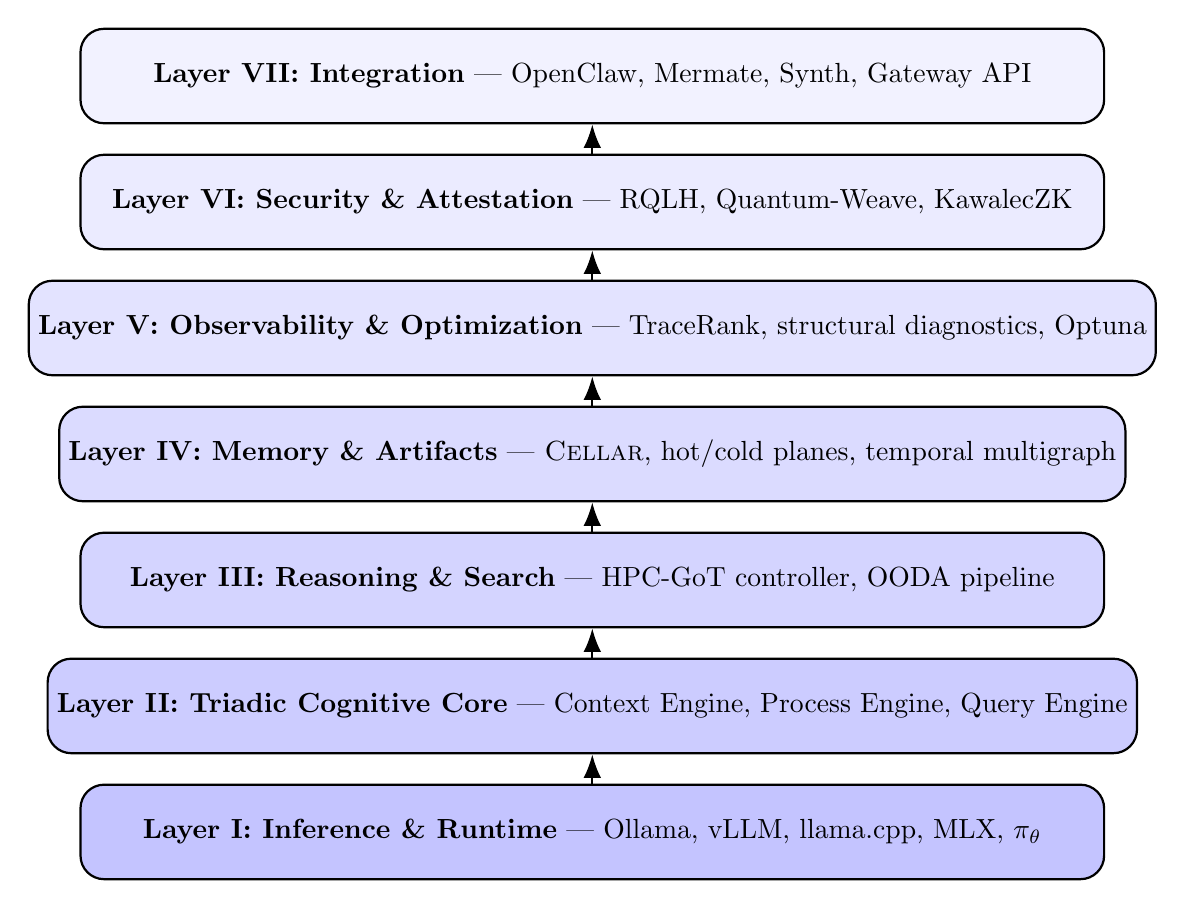
\begin{tikzpicture}[
  layer/.style={draw, rounded corners=3mm, minimum width=13cm, minimum height=1.2cm, align=center, thick},
  arrow/.style={-{Latex[length=3mm]}, thick}
]
\node[layer, fill=blue!5] (L7) at (0,0) {\textbf{Layer VII: Integration} --- OpenClaw, Mermate, Synth, Gateway API};
\node[layer, fill=blue!8] (L6) at (0,-1.6) {\textbf{Layer VI: Security \& Attestation} --- RQLH, Quantum-Weave, KawalecZK};
\node[layer, fill=blue!11] (L5) at (0,-3.2) {\textbf{Layer V: Observability \& Optimization} --- TraceRank, structural diagnostics, Optuna};
\node[layer, fill=blue!14] (L4) at (0,-4.8) {\textbf{Layer IV: Memory \& Artifacts} --- \cellar{}, hot/cold planes, temporal multigraph};
\node[layer, fill=blue!17] (L3) at (0,-6.4) {\textbf{Layer III: Reasoning \& Search} --- HPC-GoT controller, OODA pipeline};
\node[layer, fill=blue!20] (L2) at (0,-8.0) {\textbf{Layer II: Triadic Cognitive Core} --- Context Engine, Process Engine, Query Engine};
\node[layer, fill=blue!23] (L1) at (0,-9.6) {\textbf{Layer I: Inference \& Runtime} --- Ollama, vLLM, llama.cpp, MLX, $\pi_\theta$};

\foreach \i/\j in {L1/L2, L2/L3, L3/L4, L4/L5, L5/L6, L6/L7} {
  \draw[arrow] (\i) -- (\j);
}
\end{tikzpicture}
\caption{The seven-layer Opseeq architecture. Each layer depends on the layers below it.}
\label{fig:layers}
\end{figure}

% ======================================================================
\section{Layer I: Inference and Runtime}
\label{sec:inference}

The inference layer provides the raw computational substrate. It hosts one or more local language models and exposes them through standardized APIs.

\textbf{Primary engines:} Ollama (pull-and-run ergonomics, Harmony compliance), vLLM (high-throughput batching), llama.cpp (maximal portability), MLX (Apple Silicon unified memory).

\textbf{Model substrate:} Opseeq is designed around open-weight models in the 7B--21B active-parameter range, with \texttt{gpt-oss-20b} (21B parameters, 3.6B active, MoE architecture) as the canonical reference target.\footnote{Source: \texttt{tracerank.tex} \S3; \texttt{HPC-GoT.tex} \S1.}

\textbf{Deployment principle:} The inference engine is \emph{not} replaced by Opseeq. It is wrapped. Opseeq treats inference as an observable process over documented surfaces---streamed deltas, structured outputs, runtime timings---rather than as a black box producing final strings.\footnote{Source: \texttt{tracerank.tex} \S Design thesis.}

% ======================================================================
\section{Layer II: The Triadic Cognitive Core}
\label{sec:triad}

The triadic core is the cognitive center of Opseeq. It decomposes every operation into three complementary engines that jointly manage the full lifecycle from query interpretation through execution.

\subsection{Context Engine}
\label{subsec:context}

The Context Engine maintains the complete project state $s = (\req, \ctx, \out)$ using a hybrid graph-vector store.\footnote{Source: \texttt{context-engine.tex} \S1--\S4.}

\textbf{Components:}
\begin{itemize}
  \item \textbf{Context Store.} A directed intuition graph $G_\iota = (N, E)$ for structural relationships plus a vector database $D$ for semantic embeddings.
  \item \textbf{Research Module.} Detects knowledge gaps and issues targeted queries via MCP to enrich the context store.
  \item \textbf{Documentation Generator.} Traverses and formats stored context into structured reports.
\end{itemize}

\textbf{Retrieval model:}
\[
\ctxq = \mathrm{Cypher}(G_\iota, q) \cup \HNSW(v_q, D),
\]
combining structural graph traversal with semantic nearest-neighbor search in $O(\log n)$ time.

\textbf{State update:} After each prompt execution producing output $\yp$:
\[
\ctx' = \ctx \cup \{\yp\}, \quad G_\iota' = G_\iota \cup \{n_{\yp}, (n_i \to n_{\yp}) \mid n_i \in \mathrm{Prereqs}(\yp)\}, \quad D' = D \cup \{v_{\yp}\}.
\]

\subsection{Process Engine}
\label{subsec:process}

The Process Engine orchestrates workflow execution through a deterministic finite automaton enhanced with MDP-style policy optimization.\footnote{Source: \texttt{process-engine.tex} \S1--\S8.}

\textbf{DFA model:}
\[
M = (H, S, P, \delta, h_0, F),
\]
where $H$ is the set of workflow stages (Planning, Implementation, Testing, Deployment), $P$ is the prompt set, and $\delta$ defines transitions conditioned on validation:
\[
h' = \begin{cases}
\mathrm{next}(h), & \text{if } \Validate(\yp, s) = \mathrm{pass} \wedge \mathrm{StageComplete}(h, s) \\
h, & \text{otherwise.}
\end{cases}
\]

\textbf{Prompt selection policy:}
\[
\mu_h(s) = \arg\max_{p \in \mathrm{Ready}(P_h)} R(s, p),
\]
where readiness is determined by dependency completion in $G_\iota$:
\[
\mathrm{Ready}(P_h) = \{p \mid \forall n \in \mathrm{Deps}(p),\; n \in \mathrm{Completed}(\ctx)\}.
\]

\textbf{MDP formulation for adaptive optimization:}
\[
\pi^*(s) = \arg\max_\pi \mathbb{E}\left[\sum_{t=0}^\infty \gamma^t R(s_t, \pi(s_t))\right], \quad \gamma \in [0, 1).
\]

\subsection{Query Engine}
\label{subsec:query}

The Query Engine interprets queries from users, agents, or external systems and translates them into operations across the Context and Process Engines.\footnote{Source: \texttt{query-engine.tex} \S2--\S7.}

\textbf{Pipeline:}
\[
q \xrightarrow{\Parse} \mathrm{ParsedQuery} \xrightarrow{\Plan} \mathrm{ExecutionPlan} \xrightarrow{\Execute} \{y_i\} \xrightarrow{\Format} r.
\]

\textbf{N2LF Compiler:} Converts natural language to logical form:
\[
q_{\mathrm{NL}} \to \{\mathrm{intent}: i,\; \mathrm{entities}: E,\; \mathrm{structured\_ops}: O\}.
\]

\textbf{Hybrid DBMS:} The Query Engine integrates DuckDB (local analytics), Pinecone/FAISS (vector search), and Neo4j (graph traversal) behind a unified data-access abstraction:
\[
\Retrieve(q) = \mathrm{Cypher}(G_\iota, q) \cup \HNSW(v_q, D) \cup \mathrm{Analytics}(t, p).
\]

\subsection{Triadic Integration}
\label{subsec:triad_integration}

The three engines are not independent services; they are tightly coupled through shared state:
\[
\Triad(\req) = \bigl(\Context(\req),\; \Process(\req),\; \Query(\req)\bigr).
\]

The Context Engine provides memory. The Query Engine provides interpretation and data access. The Process Engine provides orchestration and execution. Every state transition in the Process Engine reads from the Context Engine and may be initiated by the Query Engine. Every query result from the Query Engine is written back into the Context Engine. This creates a closed loop of interpretation, execution, and learning.

% ======================================================================
\section{Layer III: Reasoning and Search}
\label{sec:reasoning}

\subsection{The OODA Orchestration Pipeline}
\label{subsec:ooda}

Opseeq enforces a mandatory four-phase pipeline for every non-trivial task, following the OODA (Observe--Orient--Decide--Act) pattern:\footnote{Source: \texttt{qwen-4-agents-orch.tex} \S5; \texttt{super-intel-desktop.tex} \S2.2.}

\begin{enumerate}
  \item \textbf{Observe (Elevation).} Convert raw intent into a complete, unambiguous problem statement.
  \item \textbf{Orient (Exploration).} Explore the solution space, gather evidence, propose alternatives.
  \item \textbf{Decide (Consolidation).} Reduce noise, formalize a specification, verify coherence.
  \item \textbf{Act (Execution).} Produce deliverables and execute authorized actions through guardrailed tools.
\end{enumerate}

The phases are implemented as four agent identities sharing a single base-model substrate. Differentiation is operational---through instruction overlays and routing---not through separate model weights.\footnote{Source: \texttt{qwen-4-agents-orch.tex} \S4.}

\subsection{HPC-GoT: The Bounded Reasoning Controller}
\label{subsec:hpcgot}

For tasks whose outputs admit deterministic external validation (Mermaid diagrams, PlantUML, TLA$^+$ modules), Opseeq employs HPC-GoT, a bounded typed state-transition controller.\footnote{Source: \texttt{HPC-GoT.tex} \S1--\S9.}

\textbf{Controller parameters:}
\begin{itemize}
  \item Depth cap: $\ell \in \{0, 1, 2, 3\}$
  \item Branching: at most 3 children per node
  \item Global state budget: $N = 40$
  \item Pruning threshold: $\tau = 0.85$
\end{itemize}

\textbf{Canonical validity score:}
\begin{equation}
\sigma(A, I, T) = \tfrac{1}{2}\,\SV(A, T) + \tfrac{1}{2}\,\IC(A, I),
\end{equation}
where $\SV \in \{0, 1\}$ is structural validity (external validator) and $\IC$ is invariant coverage.

\textbf{Operator algebra:} Branch, Decompose, Validate, Prune, Select, and an optional single Merge at termination.

\begin{theorem}[Termination and Boundedness]
Under the canonical schedule, HPC-GoT terminates after at most three level transitions with $|\Sigma_{\mathrm{created}}| \le 40$ and at most four LLM-mediated stages.
\end{theorem}

\noindent\textit{Source: \texttt{HPC-GoT.tex} Theorems 1--5.}

\subsection{Reconciliation: Determinism vs.\ Stochastic Inference}
\label{subsec:reconcile_determinism}

The Query Engine's Axiom 3 assumes process determinism,\footnote{\texttt{query-engine.tex} \S6.1.} while TraceRank explicitly measures run-to-run instability $D_{\mathrm{run}}$.\footnote{\texttt{tracerank.tex} \S Mathematical model.} Opseeq resolves this as follows:

\begin{remark}[Conditional Determinism]
Process determinism holds for \emph{validated} execution paths: once an output passes validation ($\Validate(\yp, s) = \mathrm{pass}$), its state-update effect is deterministic. The stochastic variability of the model's generation process is an input to TraceRank's observability layer, not a contradiction of the Process Engine's execution model.
\end{remark}

% ======================================================================
\section{Layer IV: Memory and Artifacts}
\label{sec:memory}

\subsection{The CELLAR Runtime}
\label{subsec:cellar}

\cellar{} (Cognitive Emergent Local Lakehouse Artifact Runtime) is the memory substrate of Opseeq.\footnote{Source: \texttt{cellar.tex} \S1--\S12.} Its central thesis is that a small model should not be treated as the whole of intelligence, but as a bounded policy layer governing retrieval, scheduling, selective simulation, and durable memory formation.

\textbf{Five formal layers:}

\begin{enumerate}
  \item \textbf{Policy Layer:} $\pi_\theta(o_t, m_t, b_t) \mapsto (u_t, q_t, \hat{V}_t, \hat{C}_t)$
  \item \textbf{Transition Layer:} $T_t : (s_t, a_t) \mapsto (s_{t+1}, r_t, \omega_t)$
  \item \textbf{Artifact Layer:} $\alpha_i = (x_i, y_i, p_i, c_i, t_i, h_i)$
  \item \textbf{Graph Layer:} $\graph = (V, E, \tau, \phi)$ --- typed temporal multigraph
  \item \textbf{Posterior Layer:} $P = \{p_k, \mathrm{paths}_k, \mathrm{policies}_k, \mathrm{intervals}_k\}$
\end{enumerate}

Each layer depends on the previous: inference proposes actions, actions generate transitions, transitions emit artifacts, artifacts populate the graph, and graph-grounded trajectories collapse into posterior summaries.

\subsection{Hot and Cold Storage Planes}
\label{subsec:storage}

\textbf{Hot plane $\hot$:} Transient execution-near batches, queue-local records, vectorized summaries awaiting compaction. Optimized for low-latency access and bounded lifetime.

\textbf{Cold plane $\cold$:} Immutable artifacts, manifests, indices, checkpoints, provenance records. Optimized for durability, replayability, and structured querying.

\textbf{Practical substrate:} DuckDB for local analytical queries over artifacts; LanceDB or FAISS for vector indices; Apache Arrow for columnar serialization.

\subsection{Deduplication Pipeline}
\label{subsec:dedup}

Artifact insertion proceeds through: (1) exact hash lookup, (2) semantic candidate retrieval, (3) type-aware merge-or-append decision, (4) hot-plane insertion, (5) scheduled flush to cold storage, (6) graph-edge materialization and provenance update.\footnote{Source: \texttt{cellar.tex} \S Implementation Notes.}

% ======================================================================
\section{Layer V: Observability and Optimization}
\label{sec:observability}

\subsection{TraceRank}
\label{subsec:tracerank}

TraceRank is a sidecar observability and optimization system that transforms local inference from a black-box loop into a measurable, benchmarkable, and tunable runtime.\footnote{Source: \texttt{tracerank.tex} \S1--\S14.}

\textbf{Observable transformation chain:}
\[
x \xrightarrow{T_1} h_1 \xrightarrow{T_2} \cdots \xrightarrow{T_L} h_L = z,
\]
where $h_k$ are observable stage representations and $z$ is the final trace vector.

\textbf{Concentration:}
\[
C(z) = 1 - \frac{H(z)}{\log d}, \quad H(z) = -\sum_{i=1}^d p_i \log p_i.
\]

\textbf{Graph collapse:}
\[
\gamma_{A_\tau} = 1 - \frac{\operatorname{rank}(A_\tau)}{|V_\tau|},
\]
where $A_\tau$ is the adjacency matrix of the trace graph $G_\tau$.

\textbf{Composite structural score:}
\begin{equation}
S = \omega_1 C(z) + \omega_2 \gamma_{A_\tau} + \omega_3 \kappa_{\mathrm{obs}} + \omega_4 D_{\mathrm{run}},
\end{equation}
where high $S$ indicates elevated collapse risk, narrow routing, or unstable behavior.

\textbf{Optimization objective:}
\begin{equation}
J(\theta) = \lambda_1 Q(\theta) - \lambda_2 L(\theta) - \lambda_3 M(\theta) - \lambda_4 V(\theta),
\end{equation}
balancing quality $Q$, latency $L$, memory pressure $M$, and instability $V$.

\subsection{Adapter Promotion Pipeline}
\label{subsec:adapters}

TraceRank defines four adapter states---Candidate, Validated, Shadow-tested, Promoted---with promotion requiring improvement over baseline, no schema-fidelity regression, no material latency/memory regression, and a rollback-safe shadow test.\footnote{Source: \texttt{tracerank.tex} \S Adapter and LoRA workflow.}

% ======================================================================
\section{Layer VI: Security and Attestation}
\label{sec:security}

\subsection{RQLH Consensus}
\label{subsec:rqlh}

The Relativistic Quantum Lattice Hash provides collision-resistant attestation for the assembly process:\footnote{Source: \texttt{query-rqlh.tex} \S Cryptographic Foundations.}
\[
\Pr[H(x) = H(y)] \le \left(\frac{d}{q_*}\right)^k,
\]
where $d$ is polynomial degree, $q_j$ are prime moduli, and $q_* = \min_j q_j$. This bound follows from the Schwartz--Zippel lemma applied over a CRT lattice structure.

\subsection{Quantum-Weave: Post-Quantum Data Security}
\label{subsec:quantum_weave}

For data-at-rest and data-in-transit security, Opseeq adopts the Quantum-Weave framework:\footnote{Source: \texttt{lattice-opseeq.tex} \S4--\S7.}

\begin{itemize}
  \item \textbf{Key exchange:} CRYSTALS-Kyber (M-LWE-based, quantum-resistant).
  \item \textbf{Symmetric encryption:} AES-256-GCM (128-bit effective quantum security via Grover's bound).
  \item \textbf{Integrity:} SHA-256 Merkle trees providing $O(\log n)$ verification.
  \item \textbf{Authentication:} CRYSTALS-Dilithium digital signatures on Merkle roots.
\end{itemize}

\subsection{Trust Boundary Model}
\label{subsec:trust}

Opseeq distinguishes:\footnote{Source: \texttt{super-intel-desktop.tex} \S1.}
\begin{itemize}
  \item \textbf{In-trust:} Local inference, local orchestration, formal checking, local testing, local artifact storage.
  \item \textbf{Out-of-trust (optional):} Any external model API, cloud oracle, or remote service. Used only for critique/triangulation, never for authoritative control.
\end{itemize}

% ======================================================================
\section{Layer VII: Integration --- OpenClaw, Mermate, and Synth}
\label{sec:integration}

Opseeq functions as the super-computational and orchestration framework underlying three primary application surfaces.

\subsection{OpenClaw}
\label{subsec:openclaw}

OpenClaw is the execution sandbox and agent runtime. Opseeq provides OpenClaw with:
\begin{itemize}
  \item Inference routing through the gateway API ($\texttt{/v1/chat/completions}$, $\texttt{/api/chat}$).
  \item Network policy management and sandboxed execution boundaries.
  \item MCP tool exposure for agentic control.
\end{itemize}

\subsection{Mermate}
\label{subsec:mermate}

Mermate is the architecture and specification copilot. It is the primary consumer of HPC-GoT's validator-backed reasoning for Mermaid, PlantUML/C4, and TLA$^+$ artifact generation. Opseeq provides Mermate with:
\begin{itemize}
  \item Triadic engine access for context-aware specification generation.
  \item Architecture pipeline orchestration ($\texttt{/api/architect/pipeline}$).
  \item Formal specification rendering (TLA$^+$/TypeScript).
\end{itemize}

\subsection{Synth (Synthesis-Trade)}
\label{subsec:synth}

Synth is a prediction market trading desk. Opseeq provides Synth with:
\begin{itemize}
  \item Inference routing and model access through the OpenAI-compatible gateway.
  \item Health monitoring and availability status via background polling.
  \item Integration hooks through MCP tools for AI-powered market analysis.
\end{itemize}

\subsection{Gateway Implementation}
\label{subsec:gateway}

The Opseeq gateway (currently \texttt{opseeq:latest}, v2.1.0) exposes:\footnote{Status: \textbf{Implemented}. See \texttt{service/src/index.ts}.}
\begin{itemize}
  \item OpenAI-compatible API: $\texttt{/v1/models}$, $\texttt{/v1/chat/completions}$
  \item Console-compatible API: $\texttt{/api/status}$, $\texttt{/api/chat}$, $\texttt{/api/connectivity}$
  \item MCP server: 15 tools over SSE at $\texttt{/mcp}$
  \item Multi-provider inference routing: NVIDIA NIM, OpenAI, Anthropic, Ollama
\end{itemize}

% ======================================================================
\section{Assembly and Implementation Logic}
\label{sec:assembly}

\subsection{How the System Is Constructed}

Opseeq is assembled as a set of cooperating processes coordinated by Docker Compose on a single workstation:

\begin{enumerate}
  \item \textbf{Inference engine:} Ollama or vLLM serves the base model locally.
  \item \textbf{Opseeq gateway:} Node.js/Express service providing the triadic API surface, inference routing, MCP, and application integration.
  \item \textbf{Application surfaces:} Mermate (Node.js, port 3333) and Synth (Node.js/Python, port 8420) connect to Opseeq as downstream consumers.
  \item \textbf{Storage:} Local DuckDB for analytical queries, LanceDB/FAISS for vector indices, filesystem for artifact cold storage.
\end{enumerate}

\subsection{Runtime Wiring}

At startup, the gateway:
\begin{enumerate}
  \item Parses provider configuration from environment variables.
  \item Initializes HTTP keep-alive agents for upstream connections.
  \item Starts background health polling for Mermate and Synth.
  \item Initializes timed caches for status, model lists, and service state.
  \item Registers graceful shutdown handlers (SIGTERM/SIGINT) with connection draining.
  \item Exposes the MCP server with 15 registered tools.
\end{enumerate}

\subsection{The Assembly Loop}
\label{subsec:assembly_loop}

For full-stack development tasks, Opseeq executes the assembly loop formalized in the RQLH paper:\footnote{Source: \texttt{query-rqlh.tex} \S Assembly.}

\begin{align*}
\mathrm{Assembly}(s) = \mathrm{loop}\Bigl(\;
  & p = \mathrm{select}(R, \mu(\cos)); \\
  & \yp = \mathrm{llm}(p, X = \req_p + \ctxq + \mathrm{mcp}); \\
  & \text{if } v(\yp) < \tau_v \text{ then refine}(\yp) \text{ else update}(s', G_\iota \cup \{\yp\}); \\
  & \mathrm{a2a}(\yp);\; R.\mathrm{upsert}\;\Bigr),
\end{align*}
where $v(\yp) = \mathrm{test} + \cos + \mathrm{review}$ and $\tau_v$ is the validation threshold.

% ======================================================================
\section{Temporal State Sequencing and System Behavior Over Time}
\label{sec:temporal}

Opseeq's behavior over time is governed by three interacting temporal processes:

\begin{enumerate}
  \item \textbf{Workflow state transitions:} The Process Engine's DFA advances through stages $(h, s) \xrightarrow{p} (h', s')$ as prompts execute and validate.
  \item \textbf{Memory accumulation:} The artifact graph $\graph$ grows monotonically. Hot-plane entries are periodically flushed to cold storage. The intuition graph $G_\iota$ expands with each validated output.
  \item \textbf{Observability evolution:} TraceRank's structural score $S$ evolves across runs, detecting behavioral drift. The adapter promotion pipeline moves candidates through states over time: Candidate $\to$ Validated $\to$ Shadow-tested $\to$ Promoted.
\end{enumerate}

\textbf{Convergence termination:} Following \cellar{}'s posterior convergence postulate, deep reasoning may terminate when either the hard budget is exhausted or successive posterior estimates stabilize:
\[
\mathrm{KL}(P_t \| P_{t+1}) \le \varepsilon.
\]

% ======================================================================
\section{Human-in-the-Loop and Tool-Mediated Control}
\label{sec:hitl}

\subsection{The Human Invariant Layer}

Following the APCL methodology,\footnote{Source: \texttt{super-intel-desktop.tex} \S2.1.} the human is the sole author of the immutable foundation of correctness:
\begin{itemize}
  \item \textbf{Axioms:} Non-negotiable truths and constraints.
  \item \textbf{Postulates:} Assumed properties and operating conditions.
  \item \textbf{Corollaries:} Derived constraints that must hold.
  \item \textbf{Lemmas:} Intermediate claims required for proofs.
\end{itemize}

The system traces every generated artifact back to these human-authored invariants.

\subsection{Guardrailed Tool Execution}

Tool access follows the sandbox model:\footnote{Source: \texttt{qwen-4-agents-orch.tex} \S8.}
\begin{itemize}
  \item User specifies allowed root directories at launch.
  \item All file operations resolve absolute paths and confirm containment.
  \item Subprocess commands use $\texttt{shell=False}$ with explicit timeouts.
  \item Permission escalation requires explicit user approval.
\end{itemize}

\subsection{Tiered Validation Policy}
\label{subsec:tiered_validation}

The source papers used multiple thresholds ($\tau = 0.8$ in RQLH, $\tau = 0.85$ in HPC-GoT, coverage $\ge 0.9$ in testing stage). Opseeq unifies these into a tiered policy:

\begin{center}
\begin{tabular}{lll}
\toprule
\textbf{Tier} & \textbf{Threshold} & \textbf{Application} \\
\midrule
Exploration & $\tau_e = 0.7$ & Broad-phase search, initial retrieval filtering \\
Production & $\tau_p = 0.85$ & HPC-GoT pruning, assembly validation \\
Deployment & $\tau_d = 0.9$ & Testing stage, deployment gate \\
\bottomrule
\end{tabular}
\end{center}

% ======================================================================
\section{Performance and Local Runtime Model}
\label{sec:performance}

Opseeq is designed for single-workstation deployment. Its performance model makes the following commitments:

\textbf{Inference:} The base model runs on consumer hardware (Apple Silicon with 32--64 GB unified memory, or x86 with GPU). Weight memory is approximately $\mathrm{Params} \times \mathrm{bits}/8$ bytes; practical context windows are constrained by KV-cache memory.\footnote{Source: \texttt{qwen-4-agents-orch.tex} \S10.}

\textbf{Retrieval:} $O(\log n)$ via HNSW for vector search; $O(|N| + |E|)$ for topological sort on the intuition graph.

\textbf{HPC-GoT:} $O(1)$ controller-state complexity (budget is a fixed constant $N = 40$); at most 4 LLM-mediated stages under the canonical batching contract.

\textbf{Caching:} LRU caches with timed expiry for frequently accessed state (model lists, service health, connectivity probes).

\textbf{Network:} HTTP keep-alive agents for upstream provider connections. Background polling with exponential backoff for service health.

\textbf{Optimization:} Offline multi-objective search via Optuna over the configuration space (context length, concurrency, temperature, stop conditions).

% ======================================================================
\section{Reliability and Production Constraints}
\label{sec:reliability}

\textbf{Graceful shutdown:} SIGTERM/SIGINT handlers with connection draining and configurable grace period.

\textbf{Fault tolerance:} Checkpoint-restart for workflow state; retry with exponential backoff for transient upstream failures; rollback to previous adapter/configuration baseline.

\textbf{Serverless idle:} Optional idle-timeout shutdown for resource deactivation when no active connections exist.

\textbf{Health monitoring:} $\texttt{/health}$ (basic), $\texttt{/health/ready}$ (deep readiness), and background polling of dependent services.

\textbf{Limitations:}
\begin{itemize}
  \item TraceRank does not expose hidden activations through Ollama's standard API. It uses observable rank surrogates.
  \item HPC-GoT guarantees controller-level properties, not semantic correctness.
  \item \cellar{}'s posterior quality depends on retrieval, simulation, and scoring quality.
  \item Opseeq does not claim to replace policy enforcement, moderation, or content safety systems.
\end{itemize}

% ======================================================================
\section{Final Synthesis}
\label{sec:conclusion}

Opseeq is a seven-layer intelligence architecture that transforms a developer's workstation into a sovereign, formally grounded reasoning system. Its design proceeds from a single organizing principle: \emph{the language model is the policy layer, not the system.}

Around that policy layer, Opseeq constructs:

\begin{enumerate}
  \item A \textbf{triadic cognitive core} (Context, Process, Query) that manages the complete lifecycle from interpretation through execution, grounded in hybrid graph-vector memory and formal state machines.
  \item A \textbf{bounded reasoning controller} (HPC-GoT) that structures search-and-validate over architecture artifacts with provable termination, bounded state, and external validator scoring.
  \item An \textbf{artifact-centric memory runtime} (\cellar{}) that makes expensive computation durable, typed, and replayable through a temporal multigraph over hot and cold storage planes.
  \item A \textbf{sidecar observability layer} (TraceRank) that detects structural degradation before quality visibly declines and supports gated adapter promotion.
  \item A \textbf{post-quantum attestation substrate} (RQLH and Quantum-Weave) that ensures integrity under both classical and quantum threat models.
  \item An \textbf{OODA orchestration pipeline} that enforces disciplined transformation from raw intent through verified execution.
  \item An \textbf{integration gateway} that connects OpenClaw, Mermate, and Synth through a unified, multi-provider API surface.
\end{enumerate}

The architecture is local-first but not local-only. It is formally grounded but not divorced from implementation. It is artifact-centric but not storage-obsessed. It makes the path from question to answer inspectable, replayable, and revisable---not through one model call, but through structured computational inquiry.

Opseeq does not claim omniscience. It claims something more disciplined: that a small model, embedded in a well-designed runtime, can become substantially more capable than the same model prompted in isolation. The improvement is not merely in accuracy. It is in auditability, reproducibility, safety, and the scientific integrity of the reasoning process itself.

\appendix

% ======================================================================
\section{Source Cross-Reference Matrix}
\label{app:crossref}

The following table maps each section of this master document to the source papers that contributed to it.

{\small
\begin{longtable}{p{5.5cm}p{8.5cm}}
\toprule
\textbf{Section} & \textbf{Primary Sources} \\
\midrule
\endfirsthead
\toprule
\textbf{Section} & \textbf{Primary Sources} \\
\midrule
\endhead
\S\ref{sec:introduction} Introduction & \texttt{super-intel-desktop.tex}, \texttt{tracerank.tex}, \texttt{cellar.tex} \\
\S\ref{sec:motivation} Problem Framing & \texttt{super-intel-desktop.tex} \S1, \texttt{qwen-4-agents-orch.tex} \S2 \\
\S\ref{sec:theory} Theoretical Foundations & \texttt{cellar.tex} \S3--4, \texttt{query-engine.tex} \S6, \texttt{tracerank.tex} \S5, \texttt{HPC-GoT.tex} \S4, \texttt{query-rqlh.tex} \\
\S\ref{sec:architecture} Architecture Overview & All source papers (synthesis) \\
\S\ref{sec:inference} Layer I: Inference & \texttt{tracerank.tex} \S3--6, \texttt{super-intel-desktop.tex} \S3, \texttt{qwen-4-agents-orch.tex} \S4 \\
\S\ref{sec:triad} Layer II: Triadic Core & \texttt{context-engine.tex} \S1--5, \texttt{process-engine.tex} \S1--8, \texttt{query-engine.tex} \S1--9, \texttt{query-rqlh.tex} \\
\S\ref{sec:reasoning} Layer III: Reasoning & \texttt{HPC-GoT.tex} \S1--9, \texttt{qwen-4-agents-orch.tex} \S5--6, \texttt{super-intel-desktop.tex} \S2 \\
\S\ref{sec:memory} Layer IV: Memory & \texttt{cellar.tex} \S1--12 \\
\S\ref{sec:observability} Layer V: Observability & \texttt{tracerank.tex} \S5--11 \\
\S\ref{sec:security} Layer VI: Security & \texttt{query-rqlh.tex} \S4, \texttt{lattice-opseeq.tex} \S4--7, \texttt{super-intel-desktop.tex} \S2.4 \\
\S\ref{sec:integration} Layer VII: Integration & \texttt{query-rqlh.tex} \S2, implemented gateway (\texttt{service/src/}) \\
\S\ref{sec:assembly} Assembly Logic & \texttt{query-rqlh.tex} \S Assembly, implemented gateway \\
\S\ref{sec:temporal} Temporal Sequencing & \texttt{process-engine.tex} \S4, \texttt{cellar.tex} \S6, \texttt{tracerank.tex} \S10 \\
\S\ref{sec:hitl} HITL Control & \texttt{super-intel-desktop.tex} \S2.1, \texttt{qwen-4-agents-orch.tex} \S8 \\
\S\ref{sec:performance} Performance Model & \texttt{qwen-4-agents-orch.tex} \S10, \texttt{HPC-GoT.tex} \S App.~Complexity, \texttt{tracerank.tex} \S9 \\
\S\ref{sec:reliability} Reliability & \texttt{process-engine.tex} \S7, \texttt{cellar.tex} \S11, implemented gateway \\
\bottomrule
\end{longtable}
}

\section{Unresolved Source}
\label{app:unresolved}

The source paper \texttt{agent-builder-framework.tex} was listed in the plan but does not exist in the repository at \texttt{docs/wp/}. Its intended content---an agent-builder framework specification---is partially covered by the OODA orchestration pipeline (\S\ref{subsec:ooda}), the HPC-GoT controller (\S\ref{subsec:hpcgot}), and the \cellar{} runtime (\S\ref{subsec:cellar}). If this paper is later written, its content should be integrated into Layers II--III of this master document.

\section{Notation Index}
\label{app:notation}

\begin{longtable}{p{3cm}p{11cm}}
\toprule
\textbf{Symbol} & \textbf{Meaning} \\
\midrule
\endfirsthead
$s = (\req, \ctx, \out)$ & Project state: requirements, context, outputs \\
$G_\iota = (N, E)$ & Intuition graph (task/dependency DAG) \\
$G_\tau = (V_\tau, E_\tau)$ & Trace graph (inference-stage graph) \\
$\graph = (V, E, \tau, \phi)$ & Typed temporal artifact multigraph \\
$\hot$, $\cold$ & Hot and cold storage planes \\
$\pi_\theta$ & Local policy model with parameters $\theta$ \\
$v = f(x; \theta)$ & Neural embedding function \\
$\alpha_i$ & Artifact: $(x_i, y_i, p_i, c_i, t_i, h_i)$ \\
$\sigma$ & Validity score: $\frac{1}{2}\SV + \frac{1}{2}\IC$ \\
$S$ & TraceRank structural score \\
$J(\theta)$ & Optimization objective \\
$\Sigma$ & HPC-GoT controller state \\
$N = 40$ & HPC-GoT global state budget \\
$\Ieff$ & Effective system-level intelligence \\
\bottomrule
\end{longtable}

% ======================================================================
\begin{thebibliography}{99}

\bibitem{tracerank}
D.~Kawalec, ``TraceRank v3: A Harmony-Aware Observability and Optimization Layer for gpt-oss-20b on Ollama,'' internal whitepaper, March 2026. [\texttt{tracerank.tex}]

\bibitem{sovereign}
D.~Kawalec, ``Sovereign Desktop Superintelligence: Local-First Formal-Agentic Engineering Pipeline,'' chaotic beauty LLC, March 2026. [\texttt{super-intel-desktop.tex}]

\bibitem{qwenooda}
``Qwen3.5-9B Four-Agent OODA Orchestration Framework (Version 1.0),'' March 2026. [\texttt{qwen-4-agents-orch.tex}]

\bibitem{rqlh}
D.~C.~Kawalec, ``Opseeq: A Sovereign Local-First AI Framework for Prompt-Driven, Verifiable Full-Stack Development with Relativistic Quantum Lattice Hash (RQLH) Consensus,'' September 2024. [\texttt{query-rqlh.tex}]

\bibitem{queryengine}
D.~Kawalec, ``Opseeq Query Engine and Database Management System Architecture,'' May 2025. [\texttt{query-engine.tex}]

\bibitem{processengine}
D.~Kawalec, ``The Process API Engine for Opseeq: A Formal Architecture for Orchestrating AI-Driven Development,'' May 2025. [\texttt{process-engine.tex}]

\bibitem{quantumweave}
D.~Kawalec, ``Quantum-Weave: A Lattice-Based Cryptographic Framework for Scalable and Secure Data Transmission Between DuckDB and Snowflake,'' Greybeam.ai, May 2025. [\texttt{lattice-opseeq.tex}]

\bibitem{hpcgot}
D.~Kawalec, ``HPC-GoT: A Bounded Hierarchical Reasoning Controller for Local 21B-Scale Mixture-of-Experts Models on Architectural System-Specification Tasks,'' March 2026. [\texttt{HPC-GoT.tex}]

\bibitem{contextengine}
``The Context Engine for Opseeq: A Comprehensive Design for Large-Scale AI Solution Development,'' May 2025. [\texttt{context-engine.tex}]

\bibitem{cellar}
D.~Kawalec, ``CELLAR: Cognitive Emergent Local Lakehouse Artifact Runtime,'' 2026. [\texttt{cellar.tex}]

\bibitem{bellman}
R.~Bellman, ``A Markovian Decision Process,'' \emph{J.~Math.~Mech.}, vol.~6, no.~5, 1957.

\bibitem{hnsw}
Y.~A.~Malkov and D.~A.~Yashunin, ``Efficient and Robust Approximate Nearest Neighbor Search Using HNSW,'' \emph{IEEE TPAMI}, vol.~42, no.~4, pp.~824--836, 2020.

\bibitem{wei2022chain}
J.~Wei et al., ``Chain-of-Thought Prompting Elicits Reasoning in Large Language Models,'' in \emph{NeurIPS}, 2022.

\bibitem{yao2023tree}
S.~Yao et al., ``Tree of Thoughts: Deliberate Problem Solving with Large Language Models,'' arXiv:2305.10601, 2023.

\bibitem{besta2023graph}
M.~Besta et al., ``Graph of Thoughts: Solving Elaborate Problems with Large Language Models,'' arXiv:2308.09687, 2023.

\end{thebibliography}

\end{document}
